\documentclass{lzureport}
%\usepackage{enumerate}
\usepackage[inline]{enumitem}
\usepackage{caption}
\usepackage{amsmath}
\usepackage{amssymb} % 输出 \because 和 \therefore
\usepackage{mathtools}
\usepackage{mathrsfs}
\usepackage{graphicx}
\usepackage[dvipsnames]{xcolor}  % 更全的色系
\usepackage{listings}  % 排代码用的宏包
\usepackage{tikz}  % 画图用的宏包


%%% 制作方框 $> texdoc mdframed
\usepackage[framemethod=TikZ]{mdframed}
%%%% 定理的样式
\newcounter{Thm}[section]
%\renewcommand{\theThm}{\arabic{section}.\arabic{Thm}}
\newenvironment{Thm}[1][]{
	\refstepcounter{Thm}
	\mdfsetup{
		frametitle={
			\tikz[baseline=(current bounding box.east), outer sep=0pt]
			\node[anchor=east,rectangle,fill=orange!20]
      {\strut \ifstrempty{#1}{}{~#1}};},%Theorem~\theThm\ifstrempty{#1}{}{:~#1}};},
		innertopmargin=10pt,linecolor=orange!20,
		linewidth=2pt,topline=true,
		frametitleaboveskip=\dimexpr-\ht\strutbox\relax
	}
	\begin{mdframed}[]\relax
}{\end{mdframed}}


%%%%% 证明环境
\usepackage[leftbars,color,xcolor]{changebar}
\definecolor{DeriveColor}{rgb}{.85,.2,.25}
\setlength{\changebarsep}{-3pt}
 \setlength{\changebarwidth}{2pt}

 \newenvironment{derivation}[1]
    {\cbcolor{DeriveColor}\par \vspace{10pt}
     \begin{changebar}
    \begin{enumerate}\item[]
     \noindent\textbf{#1}
     \par\vspace{5pt}\small\noindent
   } {\end{enumerate}
 \end{changebar}\par \vspace{10pt}}

 %%%%% 举例环境
\definecolor{BarColor}{rgb}{.1,.3,.6}

%\newcounter{example}[chapter] % 这里是report没有chapter,所以用section
\newcounter{example}[section]
\renewcommand{\theexample}{\thesection.\arabic{example}}
\newcommand{\exProblem}{\par\vspace{2pt}\small\noindent\noindent}
\newcommand{\exSolution}{\par\vspace{10pt}\noindent\textbf{解:} }

\newenvironment{example}
    {\cbcolor{BarColor}\par \vspace{10pt} 
	\begin{changebar}
    \begin{enumerate}\item[]
     \refstepcounter{example}\noindent\textbf{例子
     \theexample} 
	 } {\end{enumerate} 
\end{changebar}\par \vspace{8pt}}

%%% 定义颜色
% 颜色设置
\definecolor{YBXPurple}{RGB}{102,8,116}
\definecolor{YBXGreen}{RGB}{0,166,82}
\definecolor{YBXRed}{RGB}{157,41,51}
%%%%%%%%%%%%%%%%%%%%%%%%%%%%%%%%%%%%%%%%
%% listings设置
%%%%%%%%%%%%%%%%%%%%%%%%%%%%%%%%%%%%%%%%
\lstset{
	language = Python,
	backgroundcolor = \color{yellow!10},    % 背景色:淡黄
	basicstyle = \small\ttfamily,           % 基本样式 + 小号字体
	rulesepcolor= \color{gray},             % 代码块边框颜色
	breaklines = true,                  % 代码过长则换行
	numbers = left,                     % 行号在左侧显示
	numberstyle = \small,               % 行号字体
	keywordstyle = \color{blue},            % 关键字颜色
	commentstyle =\color{green!100},        % 注释颜色
	stringstyle = \color{red!100},          % 字符串颜色
	frame = shadowbox,                  % 用(带影子效果)方框框住代码块
	showspaces = false,                 % 不显示空格
	columns = fixed,                    % 字间距固定
	%escapeinside={<@}{@>}              % 特殊自定分隔符:<@可以自己加颜色@>
	morekeywords = {as},                % 自加新的关键字(必须前后都是空格)
	deletendkeywords = {compile}        % 删除内定关键字;删除错误标记的关键字用deletekeywords删!
}


\major{计算数学}
\name{甄继伟}
\title{期末复习}
\stuid{2001312001}
\college{麻省理工大学}
\date{\zhtoday}
\expname{期末复习}
\course{视觉与机器学习}


\begin{document}

\makecover

%\input{chapter/abstract.tex}

\thispagestyle{empty}
\tableofcontents
\newpage 
\setcounter{page}{1}

%%%%%%%%%%%%正文
\newpage
\section{卷积定理}
\begin{Thm}[卷积定理]
	已知两个时域(频域)信号
	$$
	\begin{aligned}
		&\mathscr{F}[f_{1}(t)] =F_{1}(f)  \\
		&\mathscr{F}[f_{2}(t)] =F_2(f)  
	\end{aligned}
	$$
	那么
	$$
	\mathscr{F}\left[f_1(t)*f_2(t)\right]=F_1(f)\cdot F_2(f)
	$$
\end{Thm}	
卷积定理指出,

\colorbox{yellow}{\color{black}\textcolor{YBXPurple}{函数卷积的傅里叶变换}是\textcolor{YBXPurple}{函数傅立叶变换的乘积}}。

具体分为时域卷积定理和频域卷积定理,

\textcolor{YBXPurple}{时域卷积定理}即\textcolor{YBXPurple}{时域}内的卷积对应频域内的乘积;

\textcolor{YBXPurple}{频域卷积定理}即\textcolor{YBXPurple}{频域}内的卷积对应时域内的乘积,两者具有对偶关系。

傅里叶变换公式:\colorbox{yellow}{\color{black}$\mathscr{F}[f(t)]=F(f)=\int_{-\infty}^{\infty}f(t)e^{-j2\pi ft}dt$}

\begin{derivation}{证明时域卷积定理}
	$
	\begin{aligned}
		\mathscr{F}[f_{1}(t)*f_{2}(t)]&=\int_{-\infty}^{\infty}f_{1}(t)*f_{2}(t)e^{-j2\pi ft}dt \\
		&=\int_{-\infty}^{\infty}\int_{-\infty}^{\infty}f_{1}(\tau)f_{2}(t-\tau)d\tau e^{-j2\pi ft}dt \\
		&=\int_{-\infty}^{\infty}\int_{-\infty}^{\infty}f_2(t-\tau)e^{-j2\pi ft}dtf_1(\tau)d\tau  \\
		&\overset{x=t-\tau}{=}\int_{-\infty}^{\infty}\int_{-\infty}^{\infty}f_2(x)e^{-j2\pi f(x+\tau)}dxf_1(\tau)d\tau \\
		&=\int_{-\infty}^{\infty}\int_{-\infty}^{\infty}f_2(x)e^{-j2\pi f\tau}e^{-j2\pi fx}dxf_1(\tau)d\tau  \\
		&=\int_{-\infty}^\infty f_2(x)e^{-j2\pi fx}dx\int_{-\infty}^\infty f_1(\tau)e^{-j2\pi f\tau}d\tau  \\
		&=F_1(f)\cdot F_2(f)
	\end{aligned}$
\end{derivation}

\newpage
\section{黎曼-勒贝格(Riemann-Lebesgue lemma)引理}
\subsection{引理内容}
设 $f(x)\in L^1(\mathbb{R})$,即 $f$ 为 $\mathbb{R}$ 上 Lebesgue 可积函数(即$f:\mathbb{R}^n\to \mathbb{C}$是一个可测函数).

使得 
$$
\|f\|_{L^1}\int_{\mathbb{R}^n}|f(x)|dx < \infty
$$

定义其 Fourier 变换

$$
\hat{f}(\xi)=\int_{\mathbf{R}}f(x)e^{\mathrm{i}\xi x}\mathrm{d}x
$$

则$\lim\limits_{|\xi|\to\infty}\hat{f}(\xi)=0.$

%%%%%%%%%%%%%%%%%%%%%%%%%
% R-L引理的证明
因为$f\in L^1(R)$,所以对于给定的$\epsilon$,都存在一个阶梯函数$f_{\epsilon}(x)$,使得
\begin{equation}\label{First}
\int_{-\infty}^{+\infty}|f(x)-f_{\epsilon}(x)|dx<\frac{\epsilon}{2},
\end{equation}
这里
$$
f_{\epsilon}(x)=\sum_{j=1}^{N}c_jZ_{(a_j,b_j)}(x),
$$
我们希望
$$
|\int_{-\infty}^{+\infty}f(x)e^{\mathrm{i}\lambda x}\mathrm{d}x|\leq \int_{-\infty}^{+\infty}|f(x)-f_{\epsilon}|e^{\mathrm{i}\lambda x}\mathrm{d}x+|\int_{-\infty}^{\infty}f_{\epsilon}(x)e^{\mathrm{i}\lambda x}dx|
$$
可以被$\frac{1}{\lambda}$控制,所以分析第二项
\begin{equation*}
	\begin{aligned}
	|\int_{-\infty}^{\infty}f_{\epsilon}(x)e^{\mathrm{i}\lambda x}\mathrm{d}x|&=|\int_{-\infty}^{\infty}\sum_{j=1}^{N}c_jZ_{(a_j,b_j)}(x)e^{-\mathrm{i}\lambda x}\mathrm{d}x|\\	
	&=|\sum_{j=1}^{N}c_j\int_{a_j}^{b_j}1\cdot e^{\mathrm{i}\lambda x}\mathrm{d}x|\\
	&=|\sum_{j=1}^{N}c_j\frac{e^{\mathrm{i}\lambda b_j}-e^{\mathrm{i}\lambda a_j}}{i\lambda}|\\
	&\leq \sum_{j=1}^{N}|c_j|\frac{|e^{\mathrm{i}\lambda b_j}|-|e^{\mathrm{i}\lambda a_j}|}{|\lambda|}\\
	&\leq \sum_{j=1}^{N}|c_j|\frac{2}{|\lambda|}\\
	&=\frac{2}{|\lambda|}\sum_{j=1}^{N}|c_j|
    \end{aligned}
\end{equation*}
而当$\lambda\to\infty$时,有
$$
\frac{2}{|\lambda|}\sum_{j=1}^{N}|c_j|\to 0,
$$
故可令$\frac{\epsilon}{2}=\frac{2}{|\lambda|}\sum_{j=1}^{N}|c_j|$,这样就$\exists N>0$,当$\lambda>N$时有
\begin{equation}\label{Second}
\frac{2}{|\lambda|}\sum_{j=1}^{N}|c_j|<\frac{\epsilon}{2}.
\end{equation}
综合\ref{First}和\ref{Second},当$\lambda>N$时就有
\begin{equation*}
	\begin{aligned}
|\int_{-\infty}^{+\infty}f(x)e^{\mathrm{i}\lambda x}\mathrm{d}x|&\leq \int_{-\infty}^{+\infty}|f(x)-f_{\epsilon}|e^{\mathrm{i}\lambda x}\mathrm{d}x+|\int_{-\infty}^{\infty}f_{\epsilon}(x)e^{\mathrm{i}\lambda x}dx|\\
&\leq \frac{\epsilon}{2}+\frac{\epsilon}{2}.
	\end{aligned}
\end{equation*}
证毕

%%%%%%%%%%%%%%%%%%%%%%%%%

\newpage
\section{吉布斯(Gibbs phenomenon)现象}
\label{sec:吉布斯现象}
\subsection{现象解释}
\label{subsec:吉布斯现象解释}
\begin{enumerate}[label=\arabic*)]
	\item 若有界变差的周期函数$f(x)$存在间端点$x_0$\\
	在不连续点处,不连续信号的的数量逐渐增多时,不连续点附近的震荡变密,但似乎没有减弱的趋势
	\item 当$N$增大,震荡靠近间端点,但是间端点最高值\textcolor{red}{保持不变}
\end{enumerate}

\begin{figure}[htbp]%位置选项
	\centering % 插图居中
	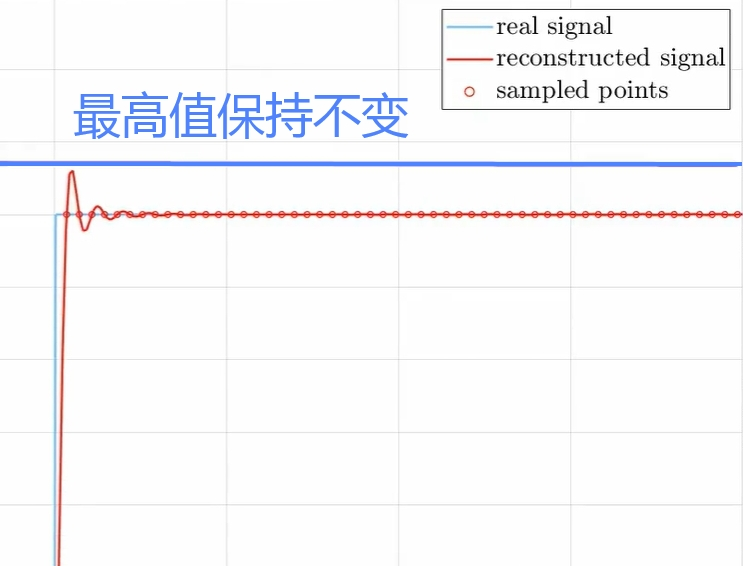
\includegraphics[width=0.6\textwidth]{figure/Gibbs现象.png}
	\caption{\label{fig:Gibbs现象}Gibbs现象}
\end{figure}

\subsection{吉布斯现象的数学解释}
\label{subsec:吉布斯现象的数学解释}
为了阐述这一现象,我们先考虑一个特例函数

$$
\varphi(x) =\left\{\begin{matrix}
	1,&0<x<\pi \\
	0,&x=0,\pm\pi \\
	-1,&-\pi<x<0
	\end{matrix}\right.
$$
 它的Fourier级数为
$$
\varphi(x) =\frac{4}{\pi}\sum_{k=1}^{\infty}\frac{\sin{(2k-1)x}}{2k-1} 
$$
有\textcolor{violet}{Jordan判别法}知其部分和$S_n(\varphi,x)$收敛到$\varphi(x),\quad x=0$是$\varphi$的间断点,我们研究部分和

$$S_{2n-1}(\varphi,x)=\frac{4}{\pi}\sum_{k=1}^{n}\frac{\sin{(2k-1)x}}{2k-1}$$

在$x=0$附近的性质,因为它是奇函数,我们只需在$[0,\pi]$上考虑.

又因为$S_{2n-1}(\varphi,\pi-x)=S_{2n-1}(\varphi,x)$,所以,我们只在$[0,\frac\pi2]$上讨论即可。

因为$S_{2n-1}(\varphi,x)$只含有限项,是连续可微的,通过逐项微商得到

$$
S_{2n-1}^{\prime}(\varphi,x)=\frac{4}{\pi}\sum_{k=1}^{n}\cos{(2k-1)x}=\frac{2}{\pi}\frac{sin2nx}{sinx}\:,x\neq0
$$
 从而我们有

$$
S_{2n-1}(\varphi,x)={\frac{2}{\pi}}\int_{0}^{x}{\frac{sin2nt}{sint}}dt
$$

容易得知

$$
S_{2n-1}^{\prime}\left(\varphi,\frac{k\pi}{2n}\right)=\frac{2}{\pi}\frac{sink\pi}{sin\frac{k\pi}{2n}}=0
$$

所以$x_k^n=\frac{k\pi}{2n}$ 是$S_{2n-1}(\varphi,x)$的极值点,当$k$为奇数时是极大值点, 当$k$为偶数时是极小值点.

$S_{2n-1}(\varphi,x)$在$x=0$右边的第一个极大值点是$x_1^n=\frac\pi{2n}$,在这点的极大值为

$$
\begin{aligned}
	S_{2n-1}\left(\varphi,{\frac{\pi}{2n}}\right)&={\frac{2}{\pi}}\int_{0}^{\frac{\pi}{2n}}{\frac{sin2nt}{sint}}dt \\
	&=\frac{2}{\pi}\int_{0}^{\pi}\frac{sint}{2nsin\frac{t}{2n}}dt\\
	&=\frac{2}{\pi}\int_{0}^{\pi}\frac{sint}{t}\frac{\frac{t}{2n}}{sin\frac{t}{2n}}dt 
\end{aligned}
$$

当$t\in(0, \pi)$有 $\begin{vmatrix}\frac{t}{2n}\\\hline sin\frac{t}{2n}\end{vmatrix}<\frac{\pi}{2}$

所以

$$
\lim_{n\to\infty}\frac{\frac{t}{2n}}{sin\frac{t}{2n}}=1
$$
当$t\in(0, \pi)$有$|\frac{\frac{t}{2n}}{sin\frac{t}{2n}}|<\frac{\pi}{2}$

故$\lim\limits_{n\to\infty}S_{2n-1}\left(\varphi,\frac{\pi}{2n}\right)=\frac{2}{\pi}\int_{0}^{\pi}\frac{sint}{t}dt=1.17898...$

以上对一个特殊的函数阐述了Gibbs现象,对于一般情形可给出如下定义:

假设函数列$\{f_n(x)\}$在$(x_0,x_0+h)$收敛于极限$f(x),h>0$,  并且$f(x_{0})$存在,假若有如下不等式成立

$$
\overline{\lim\limits_{x\to x_0+0}f_n(x)}>f(x_0+0)\left(\text{或}\underline{\lim\limits_{x\to x_0+0}f_n(x)}<f(x_0+0)\right)
$$

就说对于$\{f_n(x)\}$在点$x_0$的右半邻域有局部的Gibbs现象,对于左半邻域也有类似的定义.

\subsection{结论}
现在来说明$S_{2n-1}(\varphi,x)$收敛于$\varphi(x)$的特性。

对于充分小的$\delta>0$,$S_{2n-1}(\varphi,x)$在$\left[\delta,\frac\pi2\right]$上一致收敛于$\varphi(x)$;

而在$[0,\delta]$上其收敛是不一致的, 即不论$n$多大,都有一个点$x_1^n=\frac\pi{2n}$使$S_{2n-1}(\varphi,x)$在这点达到一个峰值,其值大约为1.17898,  它比$\varphi(x_1^n)=1$的值大约超出18%。

当$n\to\infty$时,达到峰值的点$x_1^n$趋近于零点,这种现象就是 Gibbs现象.

\begin{Thm}[帕塞瓦尔(Plancherel)定理]
\end{Thm}

\newpage
\section{香农(Shannon-Whittaker)采样定理}
\subsection{带限信号}
如果存在常数$\Omega>0$使得

$$
\widehat{f}(\omega)=0\text{,}\quad|\omega|>\Omega 
$$

成立,则称$f(t)$为\textcolor{blue}{\textbf{频率带限信号}},

当$\Omega$为满足上述等式的最小频率时$ v=\frac\Omega{2\pi}$称之为\textcolor{blue}{\textbf{Nyquist频率}},而$2v=\frac\Omega\pi$称之为\textcolor{blue}{\textbf{Nyquist速率}}。

\subsection{香农采样定理}
假设$\hat{f}(\omega)$是分段光滑的连续函数,并且$\hat{f}(\omega)=0$对于某个正数$\Omega$

当$|\omega|>\Omega$时成立,则$f=\mathcal{F}(\hat{f})$可以通过采样点$t_n=\frac{n\pi}\Omega$,$n=0$,土$1,\pm2,...$的函数值$f(t_n)$完全而唯一地确定,并可以通过下列级数展开得到

$$
f(t)=\sum_{n=-\infty}^{+\infty}f\left(\frac{n\pi}\Omega\right)\frac{sin(\Omega t-n\pi)}{(\Omega t-n\pi)}
$$

\subsection{定理证明}
\begin{derivation}{定理证明}
证明:在区间$[-\Omega,\Omega]$上对$\hat{f}(\omega)$进行Fourier级数展开

$$
\widehat{f}(\omega)=\sum_{n=-\infty}^{+\infty}c_ke^{\frac{ik\pi\omega}{\Omega}}
$$

其中

$$
c_{k}=\frac{1}{2\Omega}\int_{-\Omega}^{\Omega}\widehat{f}(\omega)e^{\frac{-ik\pi\omega}{\Omega}}d\omega 
$$

由于$\widehat{f}(\omega)=0,\quad|\omega|>\Omega$成立因此上式又可以表示为
证明: 在区间$[-\Omega,\Omega]$上对$\widehat{f}(\omega)$进行Fourier级数展开

$$
c_{k}=\frac{1}{2\Omega}\int_{-\infty}^{+\infty}\widehat{f}(\omega)e^{\frac{-ik\pi\omega}{\Omega}}d\omega=\frac{\sqrt{2\pi}}{2\Omega}f\left(-\frac{k\pi}{\Omega}\right)
$$

因此又有

$$
\hat{f}(\omega)=\frac{\sqrt{2\pi}}{2\Omega}\sum_{k=-\infty}^{+\infty}f\left(-\frac{k\pi}{\Omega}\right)e^{\frac{ik\pi\omega}{\Omega}}
$$

取$k=−k$,上式又可表示为

$$
\widehat{f}(\omega)=\frac{\sqrt{2\pi}}{2\Omega}\sum_{k=-\infty}^{+\infty}f\left(\frac{k\pi}{\Omega}\right)e^{\frac{-ik\pi\omega}{\Omega}}
$$

又由于$\hat{f}(\omega)$为分段光滑的连续函数,因此上式一致收敛,而利用Fourier变换的反演公式又得到

$$
\begin{aligned}
	f(t)&=\frac{1}{\sqrt{2\pi}}\int_{-\infty}^{+\infty}\widehat{f}(\omega)e^{i\omega t}d\omega\\
	&=\frac{1}{\sqrt{2\pi}}\int_{-\Omega}^{+\Omega}\widehat{f}(\omega)e^{i\omega t}d\omega
\end{aligned}
$$




由于$\widehat{f}(\omega)=0,\quad|\omega|>\Omega$成立因此上式又可以表示为

$$
\begin{aligned}
	f(t)&=\frac{1}{\sqrt{2\pi}}\int_{-\infty}^{+\infty}\widehat{f}(\omega)e^{i\omega t}d\omega\\
&=\frac{1}{\sqrt{2\pi}}\int_{-\Omega}^{+\Omega}\frac{\sqrt{2\pi}}{2\Omega}\sum_{k=-\infty}^{+\infty}f\left(\frac{k\pi}{\Omega}\right)e^{\frac{-ik\pi\omega}{\Omega}+i\omega t}d\omega  \\
&=\frac{1}{2\Omega}\int_{-\Omega}^{+\Omega}\sum_{k=-\infty}^{+\infty}f\left(\frac{k\pi}{\Omega}\right)e^{\frac{-ik\pi\omega}{\Omega}+i\omega t}d\omega  \\
&=\frac{1}{2\Omega}\sum_{k=-\infty}^{+\infty}\int_{-\Omega}^{+\Omega}f\left(\frac{k\pi}{\Omega}\right)e^{\frac{-ik\pi\omega}{\Omega}+i\omega t}d\omega \\
&=\frac{1}{2\Omega}\sum_{k=-\infty}^{+\infty}f\left(\frac{k\pi}{\Omega}\right)\int_{-\Omega}^{+\Omega}e^{\frac{-ik\pi\omega}{\Omega}+i\omega t}d\omega  \\
&=\frac{1}{2\Omega}\sum_{k=-\infty}^{+\infty}f\left(\frac{k\pi}{\Omega}\right)\frac{2\Omega sin(\Omega t-k\pi)}{\Omega t-k\pi} \\
&=\sum_{k=-\infty}^{+\infty}f\left(\frac{k\pi}\Omega\right)\frac{sin(\Omega t-k\pi)}{\Omega t-k\pi}
\end{aligned}
$$

定理结论成立

\end{derivation}


\begin{Thm}[Fourier变换的反演公式]
	傅里叶反演公式是经典傅里叶公式的推广。在数学中,傅里叶反演定理说,对于许多类型的函数,可以从其傅里叶变换中得到原函数。 
	
	直观地,它可以被视为,如果我们知道关于波的所有频率和相位信息,那么我们可以精确地重建原始波。
\end{Thm}

\subsection{表达式}
$$
f(t)=\sum_{n=-\infty}^{+\infty}f\left(\frac{n\pi}\Omega\right)\frac{\sin(\Omega t-n\pi)}{(\Omega t-n\pi)}
$$

\newpage
\section{张正友标定方法流程}
\subsection{相机标定}	
相机标定,就是通过实验等方法将相机模型中的未知数给解算出来。

eg:例如小孔模型我们一般需要节算出内参矩阵 fx,fy,cx,cy 以及畸变参数。

为什么要标定出这些参数呢?一个是因为每个镜头的畸变程度各不相同,通过相机标定可以校正这种镜头畸变矫正畸变,生成矫正后的图像;另一个是根据获得的图像重构三维场景。

\subsubsection{思想}
利用平面棋盘格进行相机标定的实用方法。该方法既克服了摄影标定法需要的高精度三维标定物的缺点,又解决了之前自标定法鲁棒性差的难题。

标定过程仅需使用一个打印出来的棋盘格,并从不同方向拍摄几组图片即可,任何人都可以自己制作标定图案,不仅实用灵活方便,而且精度很高,鲁棒性好。因此很快被全世界广泛采用,极大的促进了三维计算机视觉从实验室走向真实世界的进程。


\subsection{标定流程}
\begin{enumerate}[label=\arabic*)]
	\item 打印一张标定板,然后附加到一个平坦的表面上。
	\item 通过移动相机或者平面拍摄标定板各种角度的图片。
	\item 检测图片中的特征点
	\item 计算5个内部参数和所有的外部参数
	\item 通过最小二乘法先行求解径向畸变系数。
	\item 通过求最小参数值,优化所有的参数
\end{enumerate}

\subsection{解算过程}
根据上面的标定流程可知,只有第4)步骤才是真正求解的过程

首先用于标定的棋盘格是三维场景中的一个平面$\Pi$,其在成像平面的像是另一个平面$\pi$,知道了两个平面的对应点的坐标,就可以求解得到两个平面的单应矩阵$H$。\\
(其中,标定的棋盘格是特制的,其角点的坐标是已知的;图像中的角点,可以通过角点提取算法得到,这样就可以得到棋盘平面$\Pi$和图像平面$\pi$的单应矩阵$H$,即:)

$$p=K[R|t]P$$

其中$p$是像点坐标,$P$是标定的棋盘坐标,$K$是相机内参,为了不失一般性,可以在相机的内参矩阵上添加一个扭曲参数$\gamma$。即:

$$
K=\begin{bmatrix}
	f_x&\gamma&c_x\\
	0&f_y&c_y\\
   0&0&1
   \end{bmatrix}
$$

这样就可以得到下面的等式:

$$
H=K[R|t]
$$

\textbf{通过对应的点对解得$H$后,则可以通过上面的等式得到相机的内参数$K$,以及外参旋转矩阵$R$和平移向量$t$。}

设棋盘格所在的平面为世界坐标系中$Z=0$的平面,这样棋盘格的任一角点$P$的世界坐标为$(X,Y,0)$,根据小孔相机模型:

$$
s\begin{pmatrix}
	u \\
	v \\
	1
	\end{pmatrix}=K\begin{bmatrix}
	 R & t
	\end{bmatrix}\begin{pmatrix}
	X \\
	Y \\
	0 \\
	1
	\end{pmatrix}=K\begin{bmatrix}
	 r_1 & r_2 & r_3 & t
	\end{bmatrix}\begin{pmatrix}
	X \\
	Y \\
	0 \\
	1
	\end{pmatrix}=K\begin{bmatrix}
	 r_1 & r_2 &  t
	\end{bmatrix}\begin{pmatrix}
	X \\
	Y \\
	1
\end{pmatrix}
$$

再根据单应性原则:

$$
s\begin{pmatrix}
	u \\
	v \\
	1
	\end{pmatrix}=H\begin{pmatrix}
	X \\
	Y \\
	1
\end{pmatrix}
$$

根据上面两式则有:

$$
H=\begin{bmatrix}
	h_1&h_2&h_3
	\end{bmatrix}=\lambda K\begin{bmatrix}
	r_1&r_2&t
\end{bmatrix}
$$

将旋转矩阵$R$的各个列向量和平移向量$t$使用$H$的列向量表示:

$$
\begin{aligned}
	r_1&=\lambda K^{-1}h_1\\
	r_2&=\lambda K^{-1}h_2\\
	t&=\lambda K^{-1}h_3
\end{aligned}
$$

又因为,$R$是旋转矩阵,则其是正交矩阵,也就是其任意两个列向量的内积为0,列向量的模为1,则有:

$$
\begin{aligned}
	r_1^Tr_2&=0\\
	\|r_1\|&=\|r_2\|=1
\end{aligned}
$$

即

$$
\left.\left\{\begin{array}{l}h_1^TK^{-T}K^{-1}h_2=0\\h_1^TK^{-T}K^{-1}h_1=h_2^TK^{-T}K^{-1}h_2=1\end{array}\right.\right.
$$

那么对于一幅棋盘标定版的图像(一个单应矩阵)可以获得两个对内参数的约束等式。

令

$$
B=K^{-T}K^{-1}=\begin{bmatrix}B_{11}&B_{12}&B_{13}\\B_{21}&B_{22}&B_{23}\\B_{31}&B_{32}&B_{33}\end{bmatrix}
$$

矩阵$B$是一个对称矩阵,其未知量只有6个,将6个未知量写为向量的形式:

$$
b=\left[B_{11},B_{12},B_{22},B_{13},B_{23},B_{33}\right]
$$

则有:

$$
h_{i}K^{-T}K^{-1}h_{j}=h_{i}Bh_{j}=v_{ij}^{T}b
$$

其中

$$
v_{ij}=\begin{bmatrix}
	h_{i1}h_{j1}&h_{i1}h_{j2}+h_{i2}h_{j1}&h_{i2}h_{j2}&h_{i3}h_{j1}+h_{i1}h_{j3}&h_{i3}h_{j2}+h_{i2}h_{j3}&h_{i3}h_{j3}
	\end{bmatrix}^T	
$$

则约束等式有:

$$
\left.\left\{\begin{array}{l}h_1^TK^{-T}K^{-1}h_2=0\\h_1^TK^{-T}K^{-1}h_1=h_2^TK^{-T}K^{-1}h_2=1\end{array}\right.\right.\Rightarrow\left\{\begin{array}{l}v_{22}^Tb=0\\v_{11}b=v_{12}b\end{array}\right.
$$

写成矩阵的形式有:

$$
\left.\left[\begin{matrix}v_{12}^T\\v_{11}-v_{22}\end{matrix}\right.\right]b=0
$$

假如有$n$幅图像,则:

$$
Vb=0
$$

其中,$V$是一个2$n\times 6$的矩阵,$b$是一个6维向量,所以

\begin{enumerate}[label=\arabic*)]
	\item 当$n\ge 3$,可以得到$b$的唯一解;
	\item 当$n=2$,则可以假设扭曲参数$\gamma=0$作为额外的约束条件
	\item 当$n=1$,则值能计算两个相机的内参数
\end{enumerate}	


对于方程$Vb=0$可以使用SVD求得其最小二乘解。

对$VTV$进行SVD分解,其最小特征值对应的特征向量就是$Vb=0$的最小二乘解,从而求得矩阵$B$。

由于这里得到的$B$的估计值是在相差一个常量因子下得到的,所以有:

$$
B=\lambda A^{-T}A
$$

所以有

$$
\begin{cases}
	c_x=\gamma c_y/\beta-B_{13}\alpha^2/\lambda\\
	c_y=(B_{12}B_{13}-B_{11}B_{23})/(B_{11}B_{22}-B_{12}^2)\\
	\alpha=\sqrt{\lambda/B_{11}}\\
	\beta=\sqrt{\lambda B_{11}/(B_{11}B_{22}-B_{12}^2)}\\
	\gamma=-B_{12}\alpha^2\beta/\lambda\\
	\lambda=B_{33}-[B_{13}^2+c_y(B_{12}B_{13}-B_{11}B_{23})]/B_{11}
\end{cases}
$$

其中$fx =\alpha(\frac{1}{\gamma}),fy = \beta(\frac{1}{\gamma})$

为了进一步增加标定结果的可靠性,可以使用最大似然估计来优化上面估计得到的结果。

假设同一相机从$n$个不同的角度的得到了$n$幅标定板的图像,每幅图像上有$m$个像点。$M_{ij}$表示第$i$幅图像上第$j$个像点对应的标定板上的三维点,则:

$$
\hat{m}(K,R_{i},t_{i},M_{ij})=K[R\quad t]M_{ij}
$$

$\hat{m}(K,R_{i},t_{i},M_{ij})$ 表示$M_{ij}$的像点。

其中,$R_{i},t_{i}$表示第$i$幅图像对应相机的旋转矩阵和平移向量,$K$是相机的内参数。则像点$m_{ij}$的概率密度函数是:

$$
f(m_{ij})=\frac{1}{\sqrt{2\pi}}e^{\frac{-(\hat{m}(K,R_i,J_i,M_{ij})-m_{ij})^2}{\sigma^2}}
$$

构造似然函数

$$
L(A,R_i,t_i,M_{ij})=\prod_{i=1\atop j=1}^{n,m}f(m_{ij})=\frac{1}{\sqrt{2\pi}}e^{\frac{-\sum\limits_{i=1}^n\sum\limits_{j=1}^m(\hat{m}(K,R_i,J_i,M_{ij})-m_{ij})^2}{\sigma^2}}
$$

为了能够让$L$取得最大值,需要最小化下面的值

$$
\sum_{i=1}^n\sum_{j=1}^m\|\hat{m}(K,R_i,t_i,M_{ij})-m_{ij}\|^2
$$

问题变成了一个非线性优化问题,利用上面得到的解作为初始值,迭代得到最优解。这个过程就是在减少重投影误差的过程。

至此,通过张正友标定法,我们获得了相机的内参以及外参,但是畸变没有获得。张正友标定法只关注了影响较大的径向畸变。

\subsection{关于使用SVD分解法求解方程$Vb=0$的合理性的说明}
求解方程$Vb=0$的非零解可以等价于一个最小值问题:在$||b||=1$的限制下求$||Vb||$的最小值点$b$,我们可以使用拉格朗日乘子法解决该问题。

由拉格朗日乘子法,记函数
\begin{equation*}
\begin{aligned}
	f&=||Vb||-\lambda(||b||-1)\\
	 &=b^TV^TVb-\lambda(b^Tb-1)
\end{aligned}
\end{equation*}
那么使$||Vb||$取得极值的$b$和$\lambda$必然满足如下的方程组
\begin{equation*}
	\begin{aligned}
		\frac{\partial f}{\partial b}&=2V^TVb-2\lambda b=0,\\
		\frac{\partial f}{\partial \lambda}&=b^Tb-1=0,
	\end{aligned}
\end{equation*}
故使$||Vb||$取得极值的$b$必然是$V^TV$的单位特征向量之一,此时有
$$
||Vb||=b^TV^TVb=b^T\lambda b=\lambda||b||=\lambda,
$$
所以为使$||Vb||$取得极小值,$b$需取$V^TV$的最小特征值$\lambda_0$对应的特征向量$b_0$,此时$||Vb||$取得极小值$\lambda_0$(这些特征值都非负).

综上所述,对$V$做SVD分解可以得到$V^TV$的特征向量和对应的特征值,选取其中最小的特征值$\lambda_0$,其对应的特征向量$b_0$即为方程$Vb=0$的非零近似解.

\begin{Thm}[SVD分解(奇异值分解定理)]
%\reminder{\lefthand}{\qquad 对标正规矩阵 (normal matrix), 正规矩阵都可以酉对角化。这是非常好的性质。\\
%\qquad 但是非正规矩阵是否具有类似的性质呢? \\
%\qquad 注意到正规矩阵满足 $A=UDU^*$ ,其中 两个酉矩阵互为共轭转置, 我们能不能放弃这一性质,使得非正规矩阵矩阵也有类似的分解? 当然可以。}
  设 $A=(a_{ij})\in\mathbb{C}^{m\times n}(m\geq n)$, 且 $\sigma_1\geq\sigma_2\geq\cdots\sigma_r$, 则存在$m$阶和$n$ 阶酉矩阵$U$和$V$,使得 $A=UDV^*$,其中 $D=\operatorname{diag}\{\sigma_1,\cdots,\sigma_r,0,\cdots,0\}_{m\times n}$ ,
  $\sigma_1,\ldots,\sigma_r$ 称为\textcolor{blue}{\textbf{奇异值}}。 

  SVD分解步骤,如图~\ref{fig:SVD分解步骤}所示,三步可以并行进行。


\end{Thm}
\begin{figure}[hptb]
    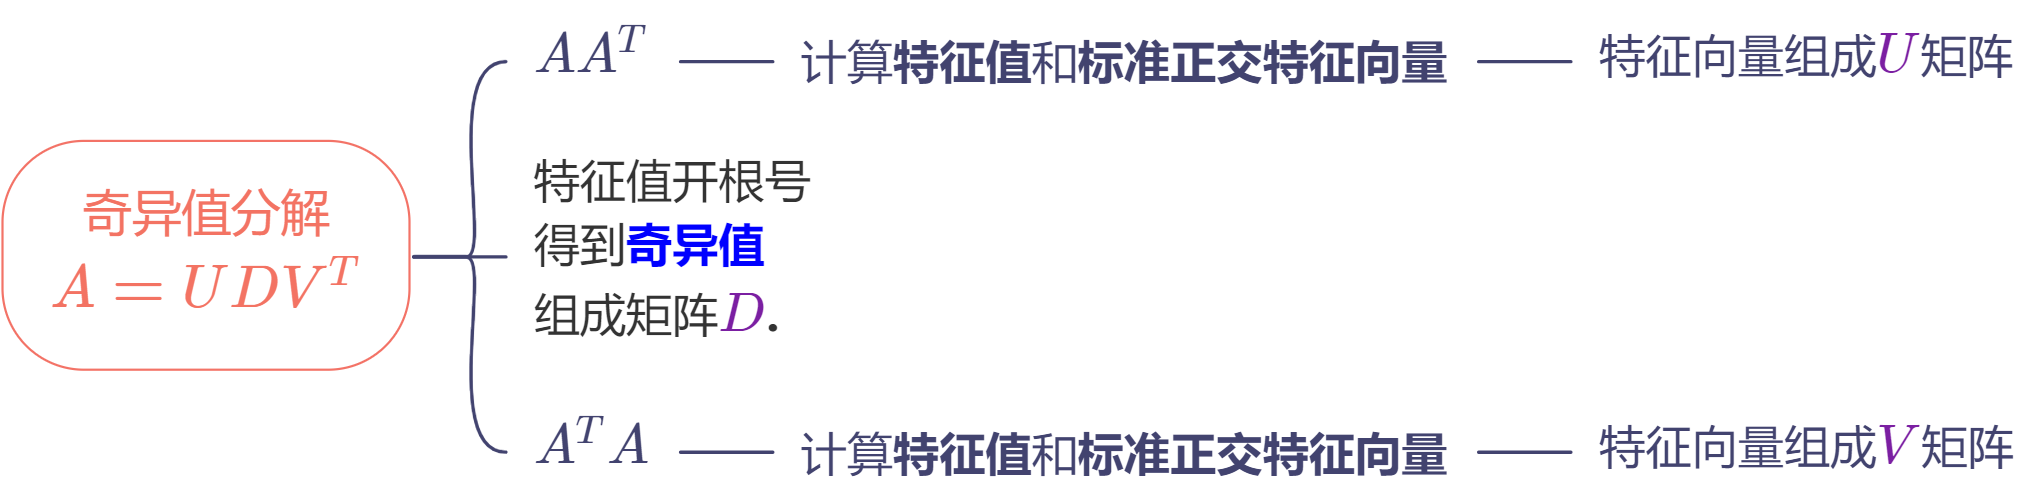
\includegraphics[width=0.8\textwidth]{figure/SVD分解步骤.png}
    \caption{\label{fig:SVD分解步骤} SVD分解步骤}
  \end{figure}


%\input{chapter/introduction.tex}
%\input{chapter/experiment.tex}

%\input{chapter/conclusion.tex}

%\input{chapter/reference.tex}
%\appendix

%\input{chapter/appendix.tex}

\end{document}
